\documentclass[11pt,aspectratio=169,hyperref={colorlinks}]{beamer}
\usetheme{Singapore}
\usecolortheme[snowy, cautious]{owl}

\usepackage[utf8]{inputenc}
\usepackage[T1]{fontenc}
\usepackage[american]{babel}
\usepackage{graphicx}
\usepackage{hyperref}
\hypersetup{
    colorlinks=true,
    urlcolor=[rgb]{0,0,0.61},
    linkcolor=[rgb]{0,0,0.61}}
\usepackage[natbib=true,style=numeric,backend=bibtex,useprefix=true]{biblatex}

%----------------------------------------------------------------------------------
\definecolor{OwlGreen}{RGB}{51,0,102} 
%----------------------------------------------------------------------------------

\setbeamertemplate{bibliography item}{}
\setbeamerfont{caption}{size=\footnotesize}
\setbeamertemplate{frametitle continuation}{}
\setcounter{tocdepth}{1}
\renewcommand*{\bibfont}{\scriptsize}
\addbibresource{lecture_3.bib}

%------------------------------------------------------------------------------------------

\usenavigationsymbolstemplate{}
\setbeamertemplate{footline}{%
    \raisebox{5pt}{\makebox{\hfill\makebox[20pt]{\color{gray}
          \scriptsize\insertframenumber}}}\hspace*{5pt}}

%------------------------------------------------------------------------------------------
\renewcommand*{\thefootnote}{\fnsymbol{footnote}}
%------------------------------------------------------------------------------------------

\author{Patrick Hall}
\title{Responsible Machine Learning\footnote{\tiny{This material is shared under a \href{https://creativecommons.org/licenses/by/4.0/deed.ast}{CC By 4.0 license} which allows for editing and redistribution, even for commercial purposes. However, any derivative work should attribute the author.}}}
\subtitle{Lecture 3: Bias Testing and Remediation}
\institute{The George Washington University}
\date{\today}


\begin{document}
	
	\maketitle
	
	\begin{frame}
	
		\frametitle{Contents}
		
		\tableofcontents{}
		
	\end{frame}


%-------------------------------------------------------------------------------
	\section{Introduction}
%-------------------------------------------------------------------------------

		\subsection*{}

		\begin{frame}
		
			\frametitle{A Responsible Machine Learning Workflow\footnote{\href{https://www.mdpi.com/2078-2489/11/3/137/htm}{\textit{A Responsible Machine Learning Workflow}}}}
			
			\begin{figure}[htb]
				\begin{center}
					\includegraphics[height=150pt]{../img/rml_diagram_lec3_hilite.png}
					\label{fig:blueprint}
				\end{center}
			\end{figure}		
					
		\end{frame}	

		\begin{frame}				
		
			\frametitle{Why Care About Bias in Machine Learning?}
			
			\begin{columns}
			
			\column{0.4\linewidth}
			\begin{itemize}\small
				\item \textbf{Responsible practice}: ML can affect millions of people! \cite{obermeyer2019dissecting}
				\item \textbf{Legal risk}: Non-compliance fines and litigation costs.
				\item \textbf{Reputational risk}: Upon encountering a perceived unethical ML system, 34\% of consumers are likely to, ``stop interacting with the company.''\footnote{\scriptsize{See: \href{https://www.capgemini.com/research/why-addressing-ethical-questions-in-ai-will-benefit-organizations/}{Why addressing ethical questions in AI will benefit organizations}.}}
			\end{itemize}
			
			\column{0.6\linewidth}
			\centering
			\begin{figure}
			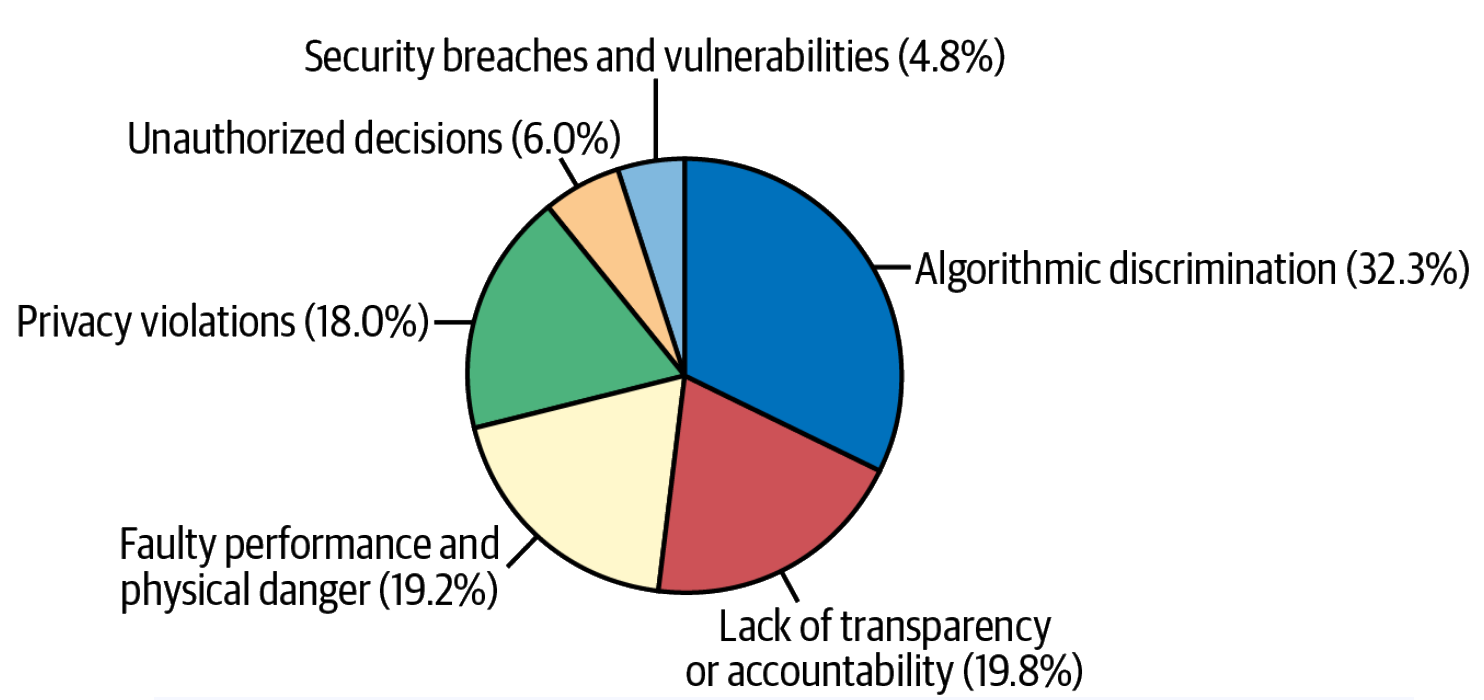
\includegraphics[scale=0.16]{../img/bias_incidents.png}
			\caption{\scriptsize{The frequency of different types of AI incidents based on a qualitative analysis of 169 publicly reported incidents between 1988 and February 1, 2021.}}
			\end{figure}
			
			\end{columns}
			
		\end{frame}

%-------------------------------------------------------------------------------
	\section{Bias in Machine Learning}
%-------------------------------------------------------------------------------
	
		\subsection*{}
	
		\begin{frame}
		
			\frametitle{What Is Bias?}			
					
			\begin{itemize}
			\item ISO defines bias as, ``the degree to which a reference value deviates from the truth.''\footnote{See: ISO 3534-1:2006.} 
			\item Because \textit{all} data and models are simplified and approximate representations of reality, \textit{all} data, statistical models, and ML models encode different types of \textit{bias}, i.e., \textbf{systematic misrepresentations of reality}.\\
			\item Oftentimes, bias is \textit{helpful}.
				\begin{itemize}
					\item{Shrunken and robust $\beta_j$ coefficients in penalized linear models.}	\end{itemize}
			\item Other types of bias can be unwanted, unhelpful, discriminatory, or illegal. 

			\end{itemize}
		
		\end{frame}
		
		\begin{frame}
		
			\frametitle{What Is Bias in ML?}	
			
		Recent authoritative work from NIST \cite{schwartz2022towards} established three main types of bias in ML: 
		
			\begin{itemize}
				\item \textbf{Systemic bias}: Sociological biases (racism, sexism, ableism, etc.) encoded in training data, design choices, or deployment choices.  
				\item \textbf{Human bias}: Cognitive mechanisms that alter human perception or cause humans to make wrong decisions.
				\item \textbf{Computational/statistical bias}: Systematically wrong model outcomes that often arise from poor data collection or model misspecification. 
			\end{itemize}
			
		The next slide will address human biases, and the remainder of this lecture focuses on systemic biases. A great deal of the class topics, e.g., explainable models, post-hoc explanation, model debugging, are meant to decrease computational/statistical bias.
			
		\end{frame}					
		
		\begin{frame}				
			
			\frametitle{What are Human Biases in ML?}		
		
			\begin{itemize}\small
				\item \textbf{Anchoring}: When a particular reference point, or \textit{anchor}, has an undue effect on people’s decisions. 
				\item \textbf{Availability heuristic}: We often confuse \textit{easy to remember} with \textit{correct}.
				\item \textbf{Confirmation bias}: People tend to prefer information that aligns with, or confirms, their existing beliefs.
				\item \textbf{Dunning-Kruger effect}: The tendency of people with low ability in a given area or task to overestimate their self-assessed ability.
				\item \textbf{Funding bias}: A bias toward highlighting or promoting results that support or satisfy the funding agency or financial supporter of a project.
				\item \textbf{Groupthink}: When people in a group tend to make nonoptimal decisions based on their desire to conform to the group or fear dissenting with the group.
				\item \textbf{McNamara fallacy}: The belief that decisions should be made based solely on quantitative information, at the expense of qualitative information or data points that aren't easily measured.
				\item \textbf{Techno-chauvinism}: The belief that technology is always the solution.		
			\end{itemize}		
		
		\end{frame}
		
		\begin{frame}				
			
			\frametitle{Legal Notions of Systemic Bias}		
			
			\begin{itemize}\small
				\item \textbf{Protected groups}: In the US, many laws and regulations prohibit discrimination based on race, sex (or gender, in some cases), age, religious affiliation, national origin, and disability status, among other categories. 
				\item \textbf{Disparate treatment}: A decision that treats an individual less favorably than similarly situated individuals because of a protected characteristic.\footnote{Concerns about disparate treatment, and more general systemic bias, are why we typically try not to use demographic markers as direct inputs to ML models.}
				\item \textbf{Disparate impact}: The result of a seemingly neutral policy or practice that disproportionately harms a protected group. 
				\item \textbf{Differential validity}: When an employment test is a better indicator of job performance for some groups than for others.
				\item \textbf{Screen out}: When a person with a disability is unable to interact with an employment assessment, and is screened out of a job or promotion by default.\footnote{See: \href{https://www.eeoc.gov/laws/guidance/americans-disabilities-act-and-use-software-algorithms-and-artificial-intelligence}{\textit{The Americans with Disabilities Act and the Use of Software, Algorithms, and Artificial Intelligence to Assess Job Applicants and Employees}} for recent EEOC statements on screenout and AI.} 
			\end{itemize}
		\end{frame}
		
		\begin{frame}				

			\frametitle{What is Systemic Bias in ML?}

				\begin{itemize}
					\item \textbf{Overt discrimination}: Using demographic information in models for the purpose of harming certain demographic groups. (Related to disparate treatment.)
					\item \textbf{Misallocation of resources}: When model \textit{outputs} disproportionately favor certain demograhic groups over others. (Related to disparate impact, often discussed as a lack of ``statistical parity.'') 
					\item \textbf{Unequal quality of service}:  When model \textit{performance} favors certain demograhic groups over others. (Related to differential validity.)
					\item \textbf{Individual or local bias}: When a model treats similar individuals differently based on demogrpahic group membership. 
				\end{itemize}

		\end{frame}

			%\frametitle{What Kinds of Discrimination Occur in ML?}	
			
			%\noindent \Large Several forms of discrimination may manifest in ML, including:
			%\begin{itemize}
				
				%\item Group disparities: 
				
				%\begin{itemize}
				
					%\item Overt discrimination against groups, i.e., \textit{disparate treatment} (DT).
					
					% More careful definition: Disparate treatment occurs when a lender treats a (potential) customer differently based on a prohibited basis, such as the person’s age, gender, or race.
					
					%\item Unintentional discrimination against groups, i.e., \textit{disparate impact} (DI).
					
					% More careful definition: Disparate impact occurs when a protected class experiences a larger share of less favorable outcomes as a result of an otherwise non-discriminatory and legitimate decision-making process. Disparate impact is not necessarily a violation of law and may be justified by a “business necessity,” such as cost or profitability. However, there may still be a violation if the lenders could have used an alternative policy or practice that had a less discriminatory effect.
					
					% All DI is discrimination, I'm not sure that all discrimination is DI.
					
					%\item Differing quality across demographic groups, i.e., \textit{differential validity}.
				
				%\end{itemize}
				
				%\item Local or individual discrimination.
				
			%\end{itemize}
		
		%\end{frame}			
		
		\begin{frame}				

			\frametitle{Who Tends to Experience Systemic Bias from ML Systems?}

			\begin{itemize} \small
				\item \textbf{Age}: 
				\begin{itemize} \scriptsize
					\item \textbf{Older people}: Those 40 and above are more likely to experience discrimination in online content; age cutoff can be older in traditional applications--employment, housing, or consumer finance.
					\item \textbf{Younger people}: Participation in Medicare or the accumulation of wealth may make older people the favored group in other scenarios.
				\end{itemize}
			 	\item \textbf{Disability}: Those with physical, mental, or emotional disabilities. 
				\item \textbf{Immigration status or national origin}: Immigrants with any immigration status, including naturalized citizens.
				\item \textbf{Language}: Those who use languages other than English or who write in non-Latin scripts.
				\item \textbf{Race and ethnicity}: Races and ethnicities other than white people, including those who identify as more than one race.
				\item \textbf{Sex and gender}: Sexes and genders other than cisgender men; in online content, women are often favored but in harmful ways (``male gaze bias''). 
				\item \textbf{Intersectional groups}: People who are in two or more of the preceding groups may experience bias or harms greater than the sum of the two broader groups.
			\end{itemize}
		\end{frame}	

		\begin{frame}[t, allowframebreaks]				

			\frametitle{What Harms Do People Experience?}

			\begin{itemize} \small
				\item \textbf{Denigration}: Derogatory or offensive content.
				\item \textbf{Erasure}: Minization or deletion of content challenging dominant social paradigms or past harms suffered by marginalized groups.
				\item \textbf{Exnomination}: Treating notions like whiteness, maleness, or heterosexuality as central human norms.
				\item \textbf{Misrecognition}: Mistaking a person’s identity or failing to recognize someone’s humanity.
				\item \textbf{Stereotyping}: Assigning characteristics to all members of a group.
				\item \textbf{Underrepresentation}: The lack of fair or adequate representation of demographic groups in model output.
				\item \textbf{Economic harms}: Reduction of the economic opportunity or value for some groups.
				\item \textbf{Physical harms}: Hurting or killing someone.  
				\item \textbf{Psychological harms}: Causing mental or emotional distress.

			\end{itemize}
		\end{frame}

		%\begin{frame}[t, allowframebreaks]				
			
			%\frametitle{How Does Systemic Bias Arise in ML?}
			
			%\noindent From poor organizational decisions, often made my homogenous groups of men with technical backgrounds.\\			
			
			%\noindent From poor experimental design:\\
			%\begin{itemize}
				%\item Asking biased questions, e.g., “can a face predict trustworthiness?”, “can demographics predict creditworthiness?”
				%\item Modeling biased phenomenon, e.g., healthcare spending vs. healthcare need. 
			%\end{itemize}
			
			%\noindent From training data:\\
			%\begin{itemize}
				%\item Incomplete or inaccurate data, e.g., under-representation of minorities. See \href{http://gendershades.org/}{Gender Shades} \cite{gender_shades}.
				%\item Accurate but differing patterns of causation, correlation, or dependency between demographic groups and past outcomes, e.g., traditional FICO credit scores.\footnote{\scriptsize{See: \url{https://shiftprocessing.com/credit-score/\#race}}}
				%\item Explicit encoding of historical social biases into training data, e.g., criminal records.
			%\end{itemize}

			%\framebreak

			%From models\\
			%\vspace{10pt}
			%\noindent \textbf{Group disparities}, i.e., different or inaccurate treatment of entire demographic groups:\\
			%\begin{itemize}
				%\item Including direct or proxy identifiers for demographic group membership, i.e., \textit{disparate treatment}.
				%\item Learning different correlations between demographic groups and favorable model outcomes, i.e., \textit{Disparate impact}.
				%\item Exhibiting different accuracies across demographic groups, i.e., \textit{differential validity}.
			%\end{itemize}
			%\vspace{5pt}
			%\noindent \textbf{Locally}, i.e., different or inaccurate treatment of similar individuals:\\
			%\begin{itemize}
				%\item Local response function or decision boundary form. 
				%\item Capacity to form local complex demographic proxies on a row-by-row basis.
			%\end{itemize}
							
		%\end{frame}

%-------------------------------------------------------------------------------
	\section{Testing for Systemic Bias in ML}
%-------------------------------------------------------------------------------

		\begin{frame}				
		
			\frametitle{Considerations for Data}

			\noindent \small General issues:\\
			\begin{itemize}\scriptsize
				\item\textbf{Representativeness}: Does the number of rows of data for each group match real demographic distributions? If no, often results in differential validity/quality of service.
				\item \textbf{Distribution of outcomes}: Are favorable outcomes ($y$ values) distributed equally across demographic groups? If no, often results in misallocation of resources/disparate impact. 
				\item \textbf{Proxies}: Do seemingly neutral features actually encode systemic bias? If yes, often results in misallocation of resources/disparate impact.   			
			\end{itemize}
			
			\noindent \small Specific examples:\\
			\begin{itemize}\scriptsize
				\item Incomplete or inaccurate data, e.g., under-representation of minorities. See \href{http://gendershades.org/}{Gender Shades} \cite{gender_shades}.
				\item Accurate but differing distributions of outcomes, correlation, or local dependencies between demographic groups and past outcomes, e.g., traditional FICO credit scores.\footnote{\scriptsize{See: \url{https://shiftprocessing.com/credit-score/\#race}}}
				\item Name or zip code acting as proxies for race.
				\item Explicit encoding of systemtic biases into training data, e.g., criminal records.
			\end{itemize}

		\end{frame}

		\begin{frame}				
		
			\frametitle{Common Test Metrics for Systemic Bias in ML}
			
			\begin{itemize}
				\item \textbf{Misallocation/disparate impact, e.g.}:			
						\begin{itemize}\small
							\item Adverse impact ratio: $\frac{\text{\% accepted}_p }{ \text{\% accepted}_c}$ 
							\item Marginal effect: $\text{\% accepted}_p - \text{\% accepted}_c$
							\item Standardized mean difference: $\frac{\bar{\hat{y}}_p - \bar{\hat{y}}_c}{\sigma_{\hat{y}}}$
						\end{itemize}
				\item \textbf{Different quality of service/validity, e.g.}: $\frac{\text{quality}_p}{\text{quality}_c}$
			\end{itemize}
			\noindent 
			\scriptsize{where, $p \equiv \text{protected group}$ and $c \equiv \text{control group}$ (often white males).}\\
			\vspace{5pt}
			\normalsize{There are many other, sometimes conflicting, mathematical definitions of discrimination. 
				See \href{https://www.youtube.com/watch?v=wqamrPkF5kk}{21 Definitions of Fairness and Their Politics}.}
			
		\end{frame}

		\begin{frame}				
		
			\frametitle{Example AIR Calculation}
			
			\centering
			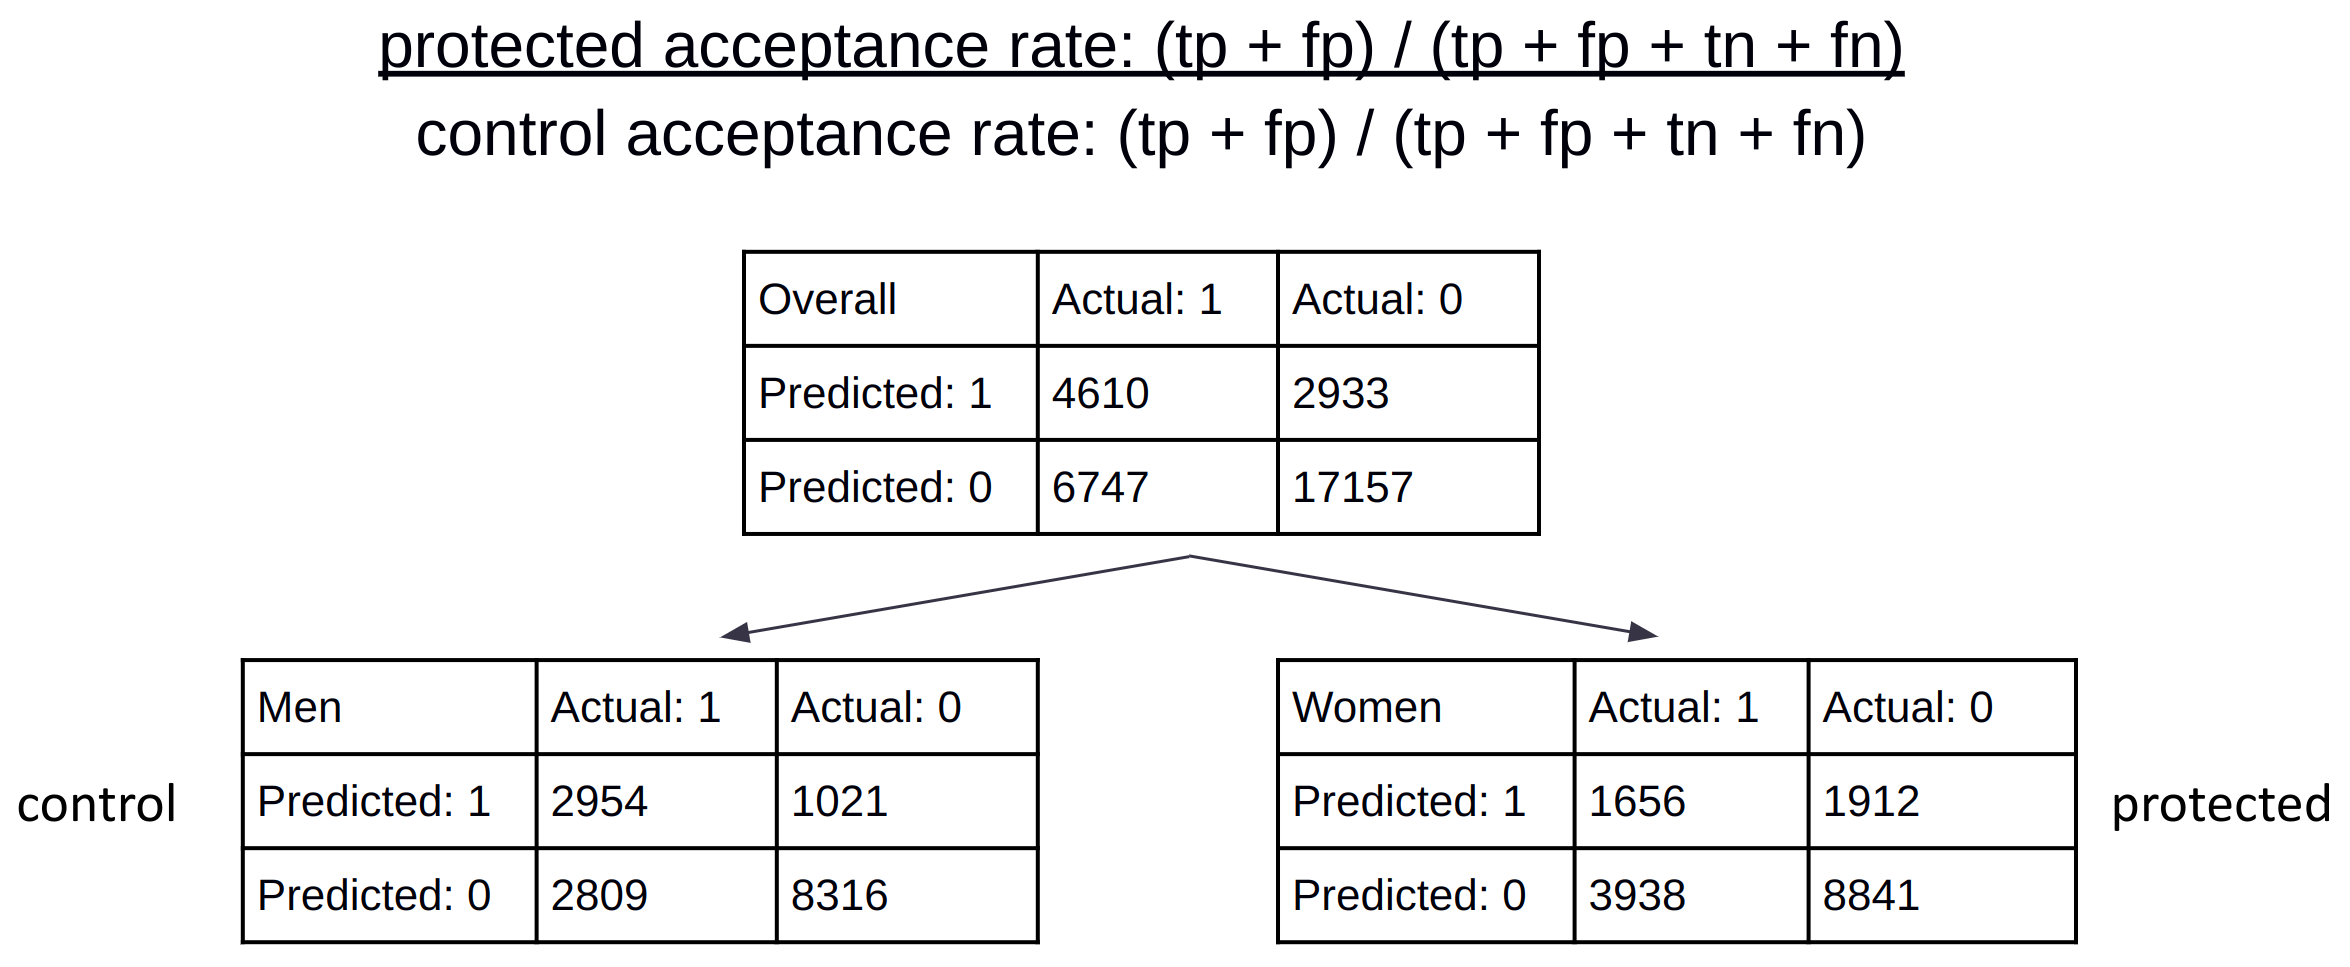
\includegraphics[scale=0.15]{../img/air1.png}
			
		\end{frame}	

		\begin{frame}				
		
			\frametitle{Example AIR Calculation}
			
			\centering
			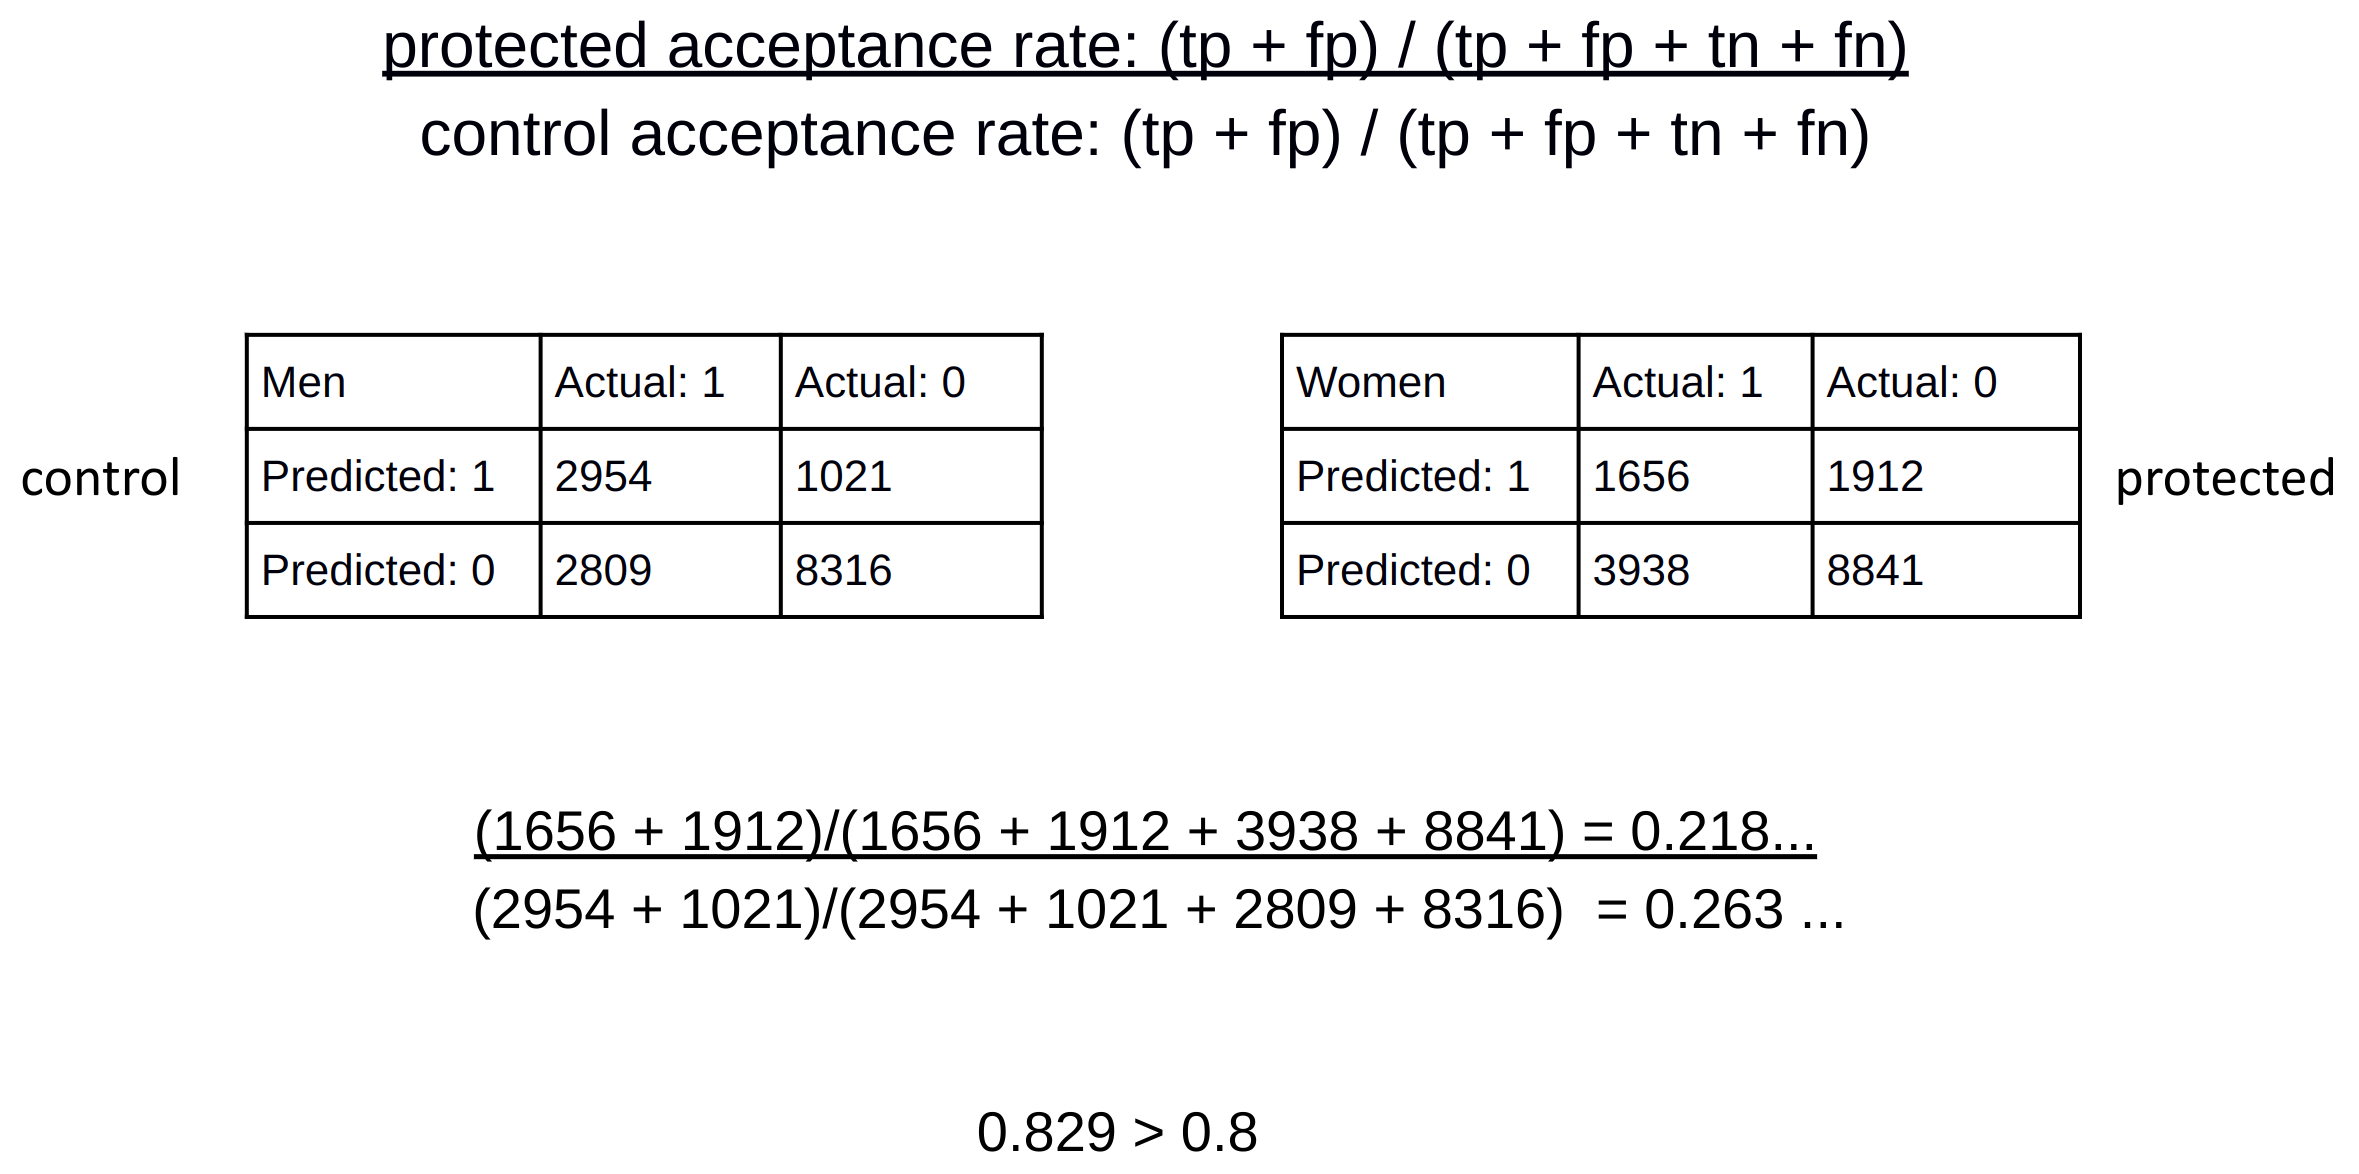
\includegraphics[scale=0.15]{../img/air2.png}
			
		\end{frame}	
		
		\begin{frame}				
		
			\frametitle{Common Test Metrics for Systemic Bias in ML}
			
			\centering
			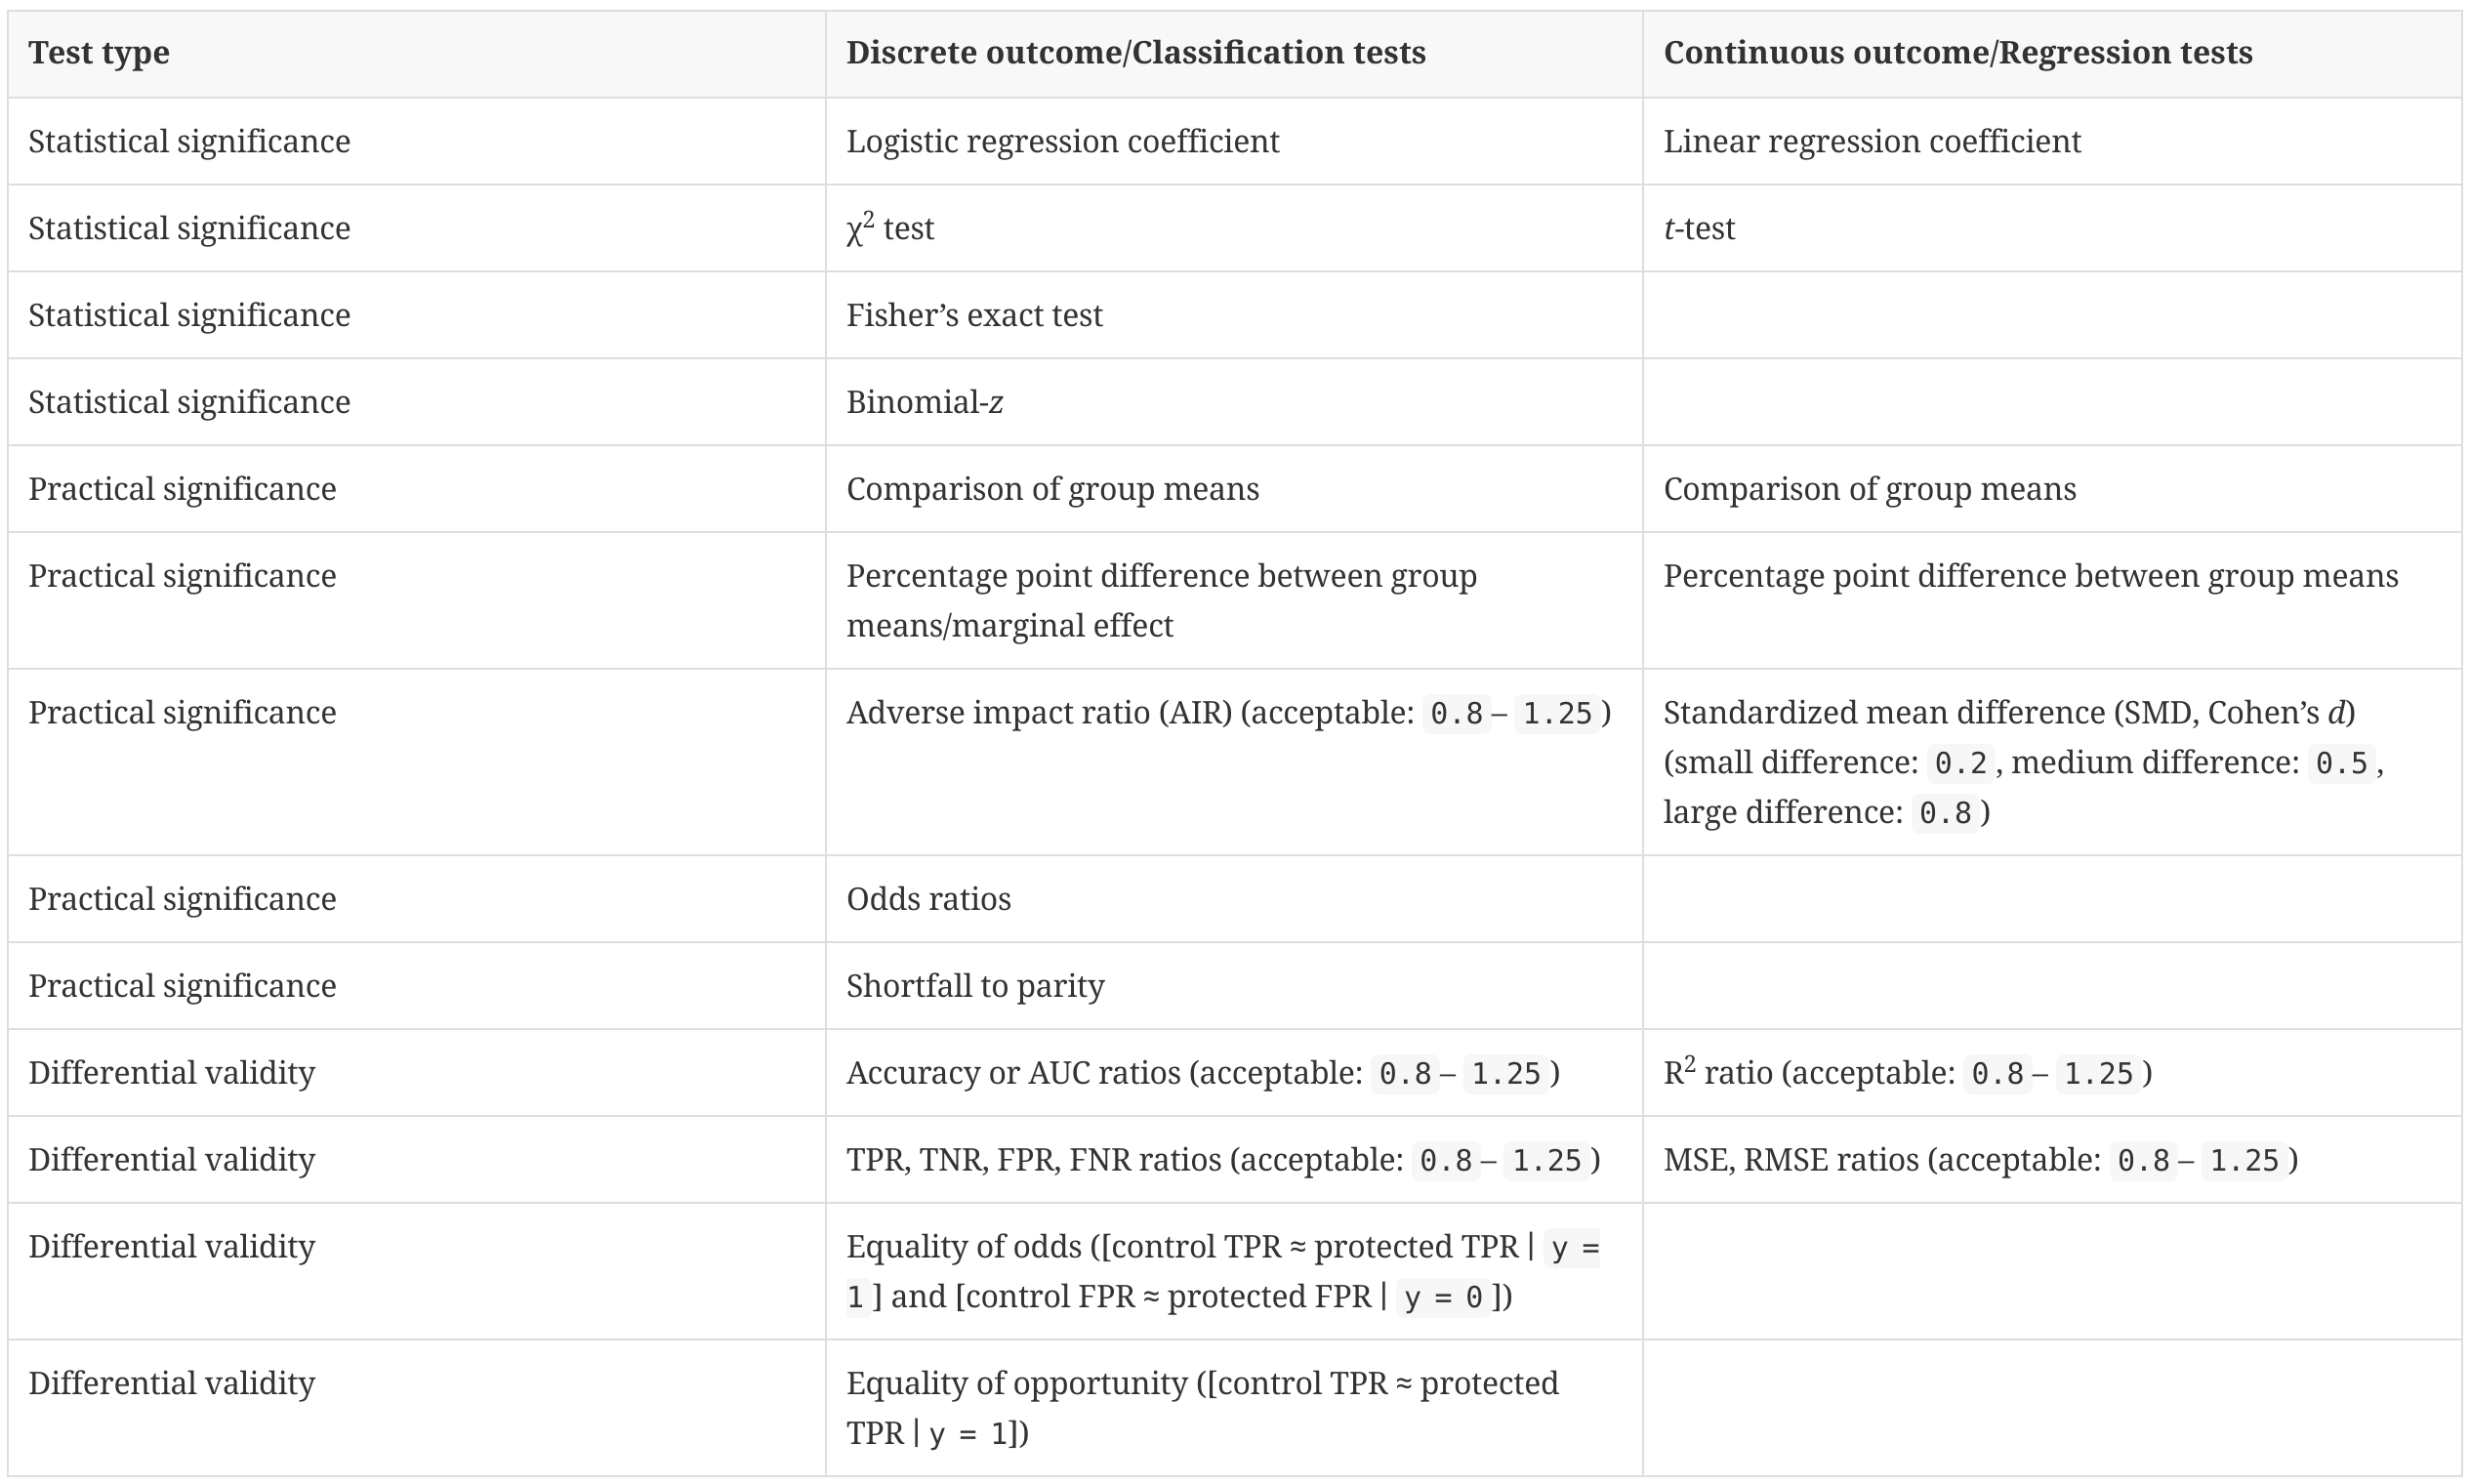
\includegraphics[scale=0.13]{../img/bias_metrics.png}
			
		\end{frame}		
		
		\begin{frame}				
	
			\frametitle{Additional Considerations for Bias Testing}
	
			\begin{itemize}\small
				\item Understand past similar incidents, via the \href{https://incidentdatabase.ai/}{AI Incident Database.}	
				\item \textbf{Adversarial models}: Use another ML model ($h_{adversary}$) to predict demographic group membership from predictions 
				($\hat{y}$) or model inputs ($X_j$). 			
				\item \textbf{Local bias}: Search around probability thresholds, apply adversarial models, apply counterfactual explanations.
				\item Understand drivers of bias with post-hoc explanation:
				\begin{itemize}
					\item To be conducted after bias is confirmed by standard tests.
					\item Be aware: lack of demographic features, fairwashing \cite{fair_washing}, and scaffolding \cite{scaffolding}. 
				\end{itemize}
				\item \textbf{Multinomial classication}: $\chi^{2}$ or equality of opportunity tests; dimension reduction on $\hat{Y}$ matrix, apply continous outcome tests.
				\item \textbf{Unsupervised learning}: Adversarial models on cluster labels or extracted features, discrete outcome tests for cluster labels, and continuous outcome tests for extracted features.
			\end{itemize}
		\end{frame}
	
%-------------------------------------------------------------------------------
	\section{Remediation}
%-------------------------------------------------------------------------------
	
		\subsection*{}

		\begin{frame}			
		
			\frametitle{How to Mitigate Systemic Bias in ML?}
			\Large \textbf{Fix the data}:
			\begin{itemize} 
				\item Collect demographically representative training data.
				\item Label and annotate data carefully.
				\item Select features judiciously.
				\item Sample and reweigh training data to minimize bias (consider group size and outcomes).\cite{kamiran2012data}
			\end{itemize}
			
		\end{frame}	
		
			
		\begin{frame}[allowframebreaks]			
		
			\frametitle{How to Mitigate Systemic Bias in ML?}			
			
			\noindent 
			\textbf{Fix the model}:
			\begin{itemize}
				\item Consider bias measures when selecting hyperparameters and cutoff thresholds.
				\item Train less biased models directly:
				\begin{itemize}
					\item Learning fair representations (LFR) and adversarial de-biasing.\cite{zemel2013learning}, \cite{zhang2018mitigating}
					\item Use dual objective functions that consider both accuracy and fairness metrics.
				\end{itemize}
				\item Edit model mechanisms to ensure less biased predictions, e.g., with \href{https://github.com/interpretml/interpret}{GA2M/EBM} models.
			\end{itemize}	
			
			\framebreak
			\centering
			\begin{figure}
			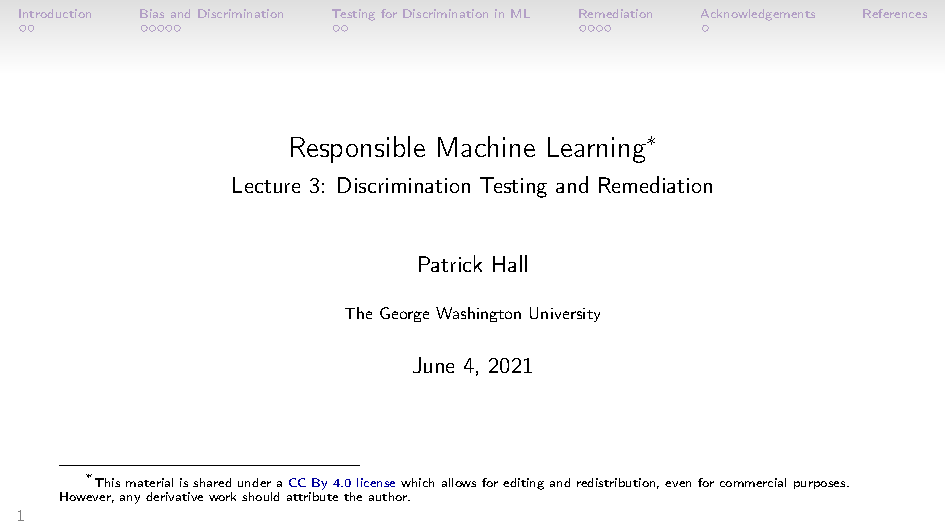
\includegraphics[scale=0.085]{../img/lecture_3.png}
			\caption{An example of considering bias measures in model selection.}
			\end{figure}
			
		\end{frame}	
		
		\begin{frame}[allowframebreaks]			
		
			\frametitle{How to Mitigate Systemic Bias in ML?}					
			
			\noindent \Large \textbf{Fix the predictions}: 
			\begin{itemize}
				\item Balance model predictions, e.g., reject-option classification.\cite{kamiran2012decision}\footnote{Re-balancing predictons based on protected class information may give rise to risks relating to disparate treatment, reverse discrimination, or unapproved affirmative action.}	
				\item Correct or override predictions with model assertions or appeal mechansims.\cite{hall2019guidelines}, \cite{kangdebugging}
			\end{itemize}
			
		\end{frame}
	
		\begin{frame}
		
			\frametitle{How to Mitigate Systemic Bias in ML?}		
			
			\begin{columns}
			
			\column{0.5\linewidth}
				\begin{itemize}
					\item Fix organizational processes/apply governance: Lecture 6.
					\item Apply the scientific method and experimental design to ML systems. 
					\item Increase demographic and professional diversity in ML teams. 
					
				\end{itemize}
			
			\column{0.5\linewidth}
				\centering
				\noindent As part of a responsible ML workflow.\\
				\vspace{10pt}
				\includegraphics[scale=0.06]{../img/rml_diagram_no_hilite.png}
			
			\end{columns}			
			
		\end{frame}		
		
%-------------------------------------------------------------------------------
	\section{Acknowledgements}
%-------------------------------------------------------------------------------

	\subsection*{}
	
	\begin{frame}
	
		\frametitle{Acknowledgements}
		
		This presentation borrows heavily from the expertise of Nicholas Schmidt of \href{https://www.bldsllc.com/}{BLDS, LLC}, a leading fair lending compliance firm.\\
		\vspace{10pt}		
		Thanks to Lisa Song for her continued assistance in developing these course materials.\\
		\vspace{10pt}
		Some materials \copyright\hspace{1pt}Patrick Hall and the H2O.ai team 2017-2020.  

	\end{frame}	
	
%-------------------------------------------------------------------------------
%	References
%-------------------------------------------------------------------------------

	\begin{frame}[t, allowframebreaks]
	
		\frametitle{References}
		\printbibliography
		
	\end{frame}

\end{document}